\documentclass[a4paper,12pt]{article}

\usepackage{amsmath,amssymb,amsfonts,gensymb,mathtext,enumerate,float,cite}
\usepackage[T2A]{fontenc}
\usepackage[utf8]{inputenc}
\usepackage[english,russian]{babel}
\usepackage{indentfirst}
\usepackage[unicode=true]{hyperref}
\usepackage{multirow}
\usepackage{array}	
\usepackage[dvips]{graphicx}
\usepackage{xymtexpdf}
\usepackage{cmap}
\graphicspath{{figures/}}



\usepackage{setspace}
% полуторный интервал
\onehalfspacing
\usepackage[14pt]{extsizes}

\hypersetup{
pdfborder={0 0 0},
pdfauthor={Khaibrakhmanov Artur Ilnurovich},
pdftitle={Diploma},
}

\usepackage{geometry}\geometry{left=3cm}
\geometry{right=2cm}
\geometry{top=2cm}
\geometry{bottom=2.5cm}

\numberwithin{equation}{section}
\numberwithin{figure}{section}
\numberwithin{table}{section}

\setcounter{tocdepth}{4}
\setcounter{secnumdepth}{4}



\RequirePackage{caption}
\DeclareCaptionLabelSeparator{defffis}{ -- }
\captionsetup{justification=centering,labelsep=defffis}
\usepackage{subfigure}
%\usepackage{subcaption}
\renewcommand{\thesubfigure}{(\asbuk{subfigure})}
\begin{document}
\righthyphenmin=20
\renewcommand{\figurename}{Рисунок}
\begin{titlepage}
\newpage

\begin{center}

\textbf{Московский государственный университет\\ имени М.В. Ломоносова}\\
\textbf{Химический факультет}\\
\text{Кафедра физической химии}\\
\text{Лаборатория строения конденсированных систем}
\end{center}
\vspace{1cm}


\vspace{8em}
\begin{center}
\textsc{\textbf{Хайбрахманов Артур Ильнурович}}
\vspace{1cm}


\textsc{\textbf{\large Применение методов ИИ для решения задач рентгенодифракционных исследований}}


\vspace{1em}

\textsc{Дипломная работа}
\end{center}
\vspace{7em}
\begin{flushright}
Научный руководитель:\\
к.\,х.\,н., с.\,н.\,с. Дмитриенко А.\,О.

д.\,х.\,н., доцент Лысенко К.\,С.

\end{flushright}

\vspace{\fill}

\begin{center}
Москва, 2025
\end{center}

\end{titlepage}

\setcounter{page}{2}
\renewcommand{\contentsname}{Оглавление}
\sloppy{
\tableofcontents

}
\newpage
\section*{Список использованных сокращений}
\addcontentsline{toc}{section}{Список использованных сокращений}
ВУФ --- вакуумный ультрафиолет

ИК --- инфракрасный

КР --- катион-радикал

ПАУ --- полициклические ароматические углеводороды

СТВ --- сверхтонкое взаимодействие

СТС --- сверхтонкая структура

УФ --- ультрафиолетовый

ЭПР --- электронный парамагнитный резонанс

Ng --- noble gas (обозначение атома благородного газа)
\section*{Введение}
\addcontentsline{toc}{section}{Введение}

Был предложен подход, который может позволить ab initio решить проблему фаз в рентгенодифракционных исследованиях. Создан генератор синтетических дифракционных данных, который может быть использован для решения прикладных задач с использованием машинного обучения. Представлен автоматизированный контейнер, позволяющий проводить воспроизводимые эксперименты по решению задачи в рамках предложенного подхода. Были разработаны модели FFT\_UNet и XRD\_Transformer, учитывающие физическую специфику задачи, проведен сравнительный анализ и интерпретация их работы на реальных данных. 


Решение проблемы фаз является важной задачей рентгеноструктурного анализа, особенно актуальной для белковой кристаллографии ввиду отсутствия ab initio решений в этой области. Методы машинного обучения способны преодолеть данную задачу. Предлагается увеличивать разрешение дифракционной картины, предсказывая моделью машинного обучения дальние отражения по ближним, что позволит решить проблему фаз ab initio для биомолекул. В работе разработан генератор синтетических рентгенодифракционных данных, который может быть использован для решения прикладных задач методами ИИ, и пайплайн для проведения воспроизводимых экспериментов для решения задачи в рамках предложенной методологии. Также были разработаны модели FFT\_UNet и XRD\_Transformer, подходящие под специфику задачи; проведены их сравнительный анализ и интерпретация их работы с помощью GradCAM и связей внимания. Было показано и обосновано, что методы глубокого обучения способны считывать кристаллографические связи и законы в рентгенодифракционных данных, но их точности численного восстановления амплитуд структурных факторов не хватает для решения проблемы фаз в рамках предложенной методологии. 

\chapter{Literature Review}

\section{Theoretical Background}
[Discuss the key theories and concepts relevant to your research]

\section{Current State of Research}
[Review and analyze existing research in your field]

\section{Research Gap}
[Identify and explain the gaps in current research that your work addresses]

\section{Summary}
[Summarize the key findings from literature and their relevance to your work] 
\section{Методика решения}

\subsection{Подход}

В работе было предложено предсказывать амплитуды структурных факторов дифракционных максимумов, которые нельзя получить из эксперимента, по известным из того же эксперимента. После предсказания достаточного количества отражений, разрешения данных должно хватить для определения фаз и расчета электронной плотности одним из рутинных ab initio методов, в качестве которого был выбран метод, реализованный в комплексе программ SHELXTL PLUS \cite{sheldrick_shelxt_2015} (схема представлена на рис. \ref{schema}). Разрешение~--- минимальное межплоскостное расстояние из набора дифракционных максимумов структуры \cite{girolami_x-ray_2016}.

\begin{figure}[H]
	\centering
	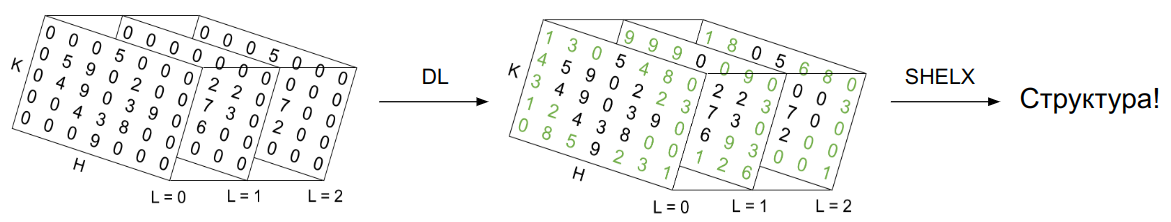
\includegraphics[width=1\textwidth]{figures/schema.png}\hfill
	\caption{Схема решения проблемы фаз с помощью методов глубокого обучения (DL). Дифракционные картины (тензоры отражений $\textbf{F}$) представлены в виде параллелепипедов}
	\label{schema}
\end{figure}

Дифракционные отражения являются точками обратного пространства, каждое из них можно однозначно описать индексами Миллера (h, k, l). Тогда дифракционную картину можно описать трехмерным тензором $\textbf{F}\in \mathbb{R}^{H\times K\times L}$, в котором записаны амплитуды каждого отражения: $\textbf{F}[h, k, l] = F (h,k,l)$. В точках, где не зарегистрированы дифракционные максимумы, в тензоре записаны нули. Таким образом, задача сводится к восстановлению трехмерного тензора. Также значения в каждом тензоре были отнормированы в диапазон 0--1. Получение результата (inference) моделей глубокого обучения должен выглядеть следующим образом: на вход подается тензор с рентгенодифракционными экспериментальными данными, на выходе должен быть тензор с амплитудами дополнительных отражений. В ходе обучения планируется научить модель восстанавливать тензор отражений по данным органических молекул. 

В работе также была проведена обработка после получения результата моделью (постпроцессинг), не входящая в обучение и включающая в себя учёт систематических погасаний --- "зануления" некоторых значений структурных факторов, что определяется симметрией структуры; в ходе обучения происходит явное восстановления части тензора, которую не нужно предсказывать.
Эффективность предсказания обученных моделей глубокого обучения проверялась на тестовой части синтетического датасета, а также тестовой части рентгенодифракционных данных моноклинных структур из CSD (Кембриджской Базы Структурных данных).

\subsection{Рентгенодифракционные данные}

Было разработано программное обеспечение, позволяющее генерировать случайные структуры и рассчитывать для них рентгенодифракционные данные (\url{github.com/blackwood168/xrd_simulator}). С помощью открытой библиотеки на языке Python CCTBX (Computational Crystallography Toolbox) \cite{grosse-kunstleve_computational_2002} создаются кристаллические решетки, в которых случайным образом с учётом симметрии расставляются случайные атомы. Для получаемых синтетических структур реализованы расчёт дифракционной картины~--- индексов и структурных факторов отражений, вычисление порошковой дифрактограммы (реализована профильная функция Псевдо--Войдта \cite{david_powder_1986} и осевая расходимость рентгеновского пучка, рис. \ref{pxrd}), а также карты Паттерсона. Нужный расчет выбирает пользователь исходя из своей текущей задачи.   Также генератор поддерживает последующий расчет данных рентгеновской порошковой дифракции. Созданное ПО может быть полезно для решения прикладных задач рентгенодифракционных исследований кристаллов с помощью методов машинного обучения. 


\begin{figure}[H]
	\centering
	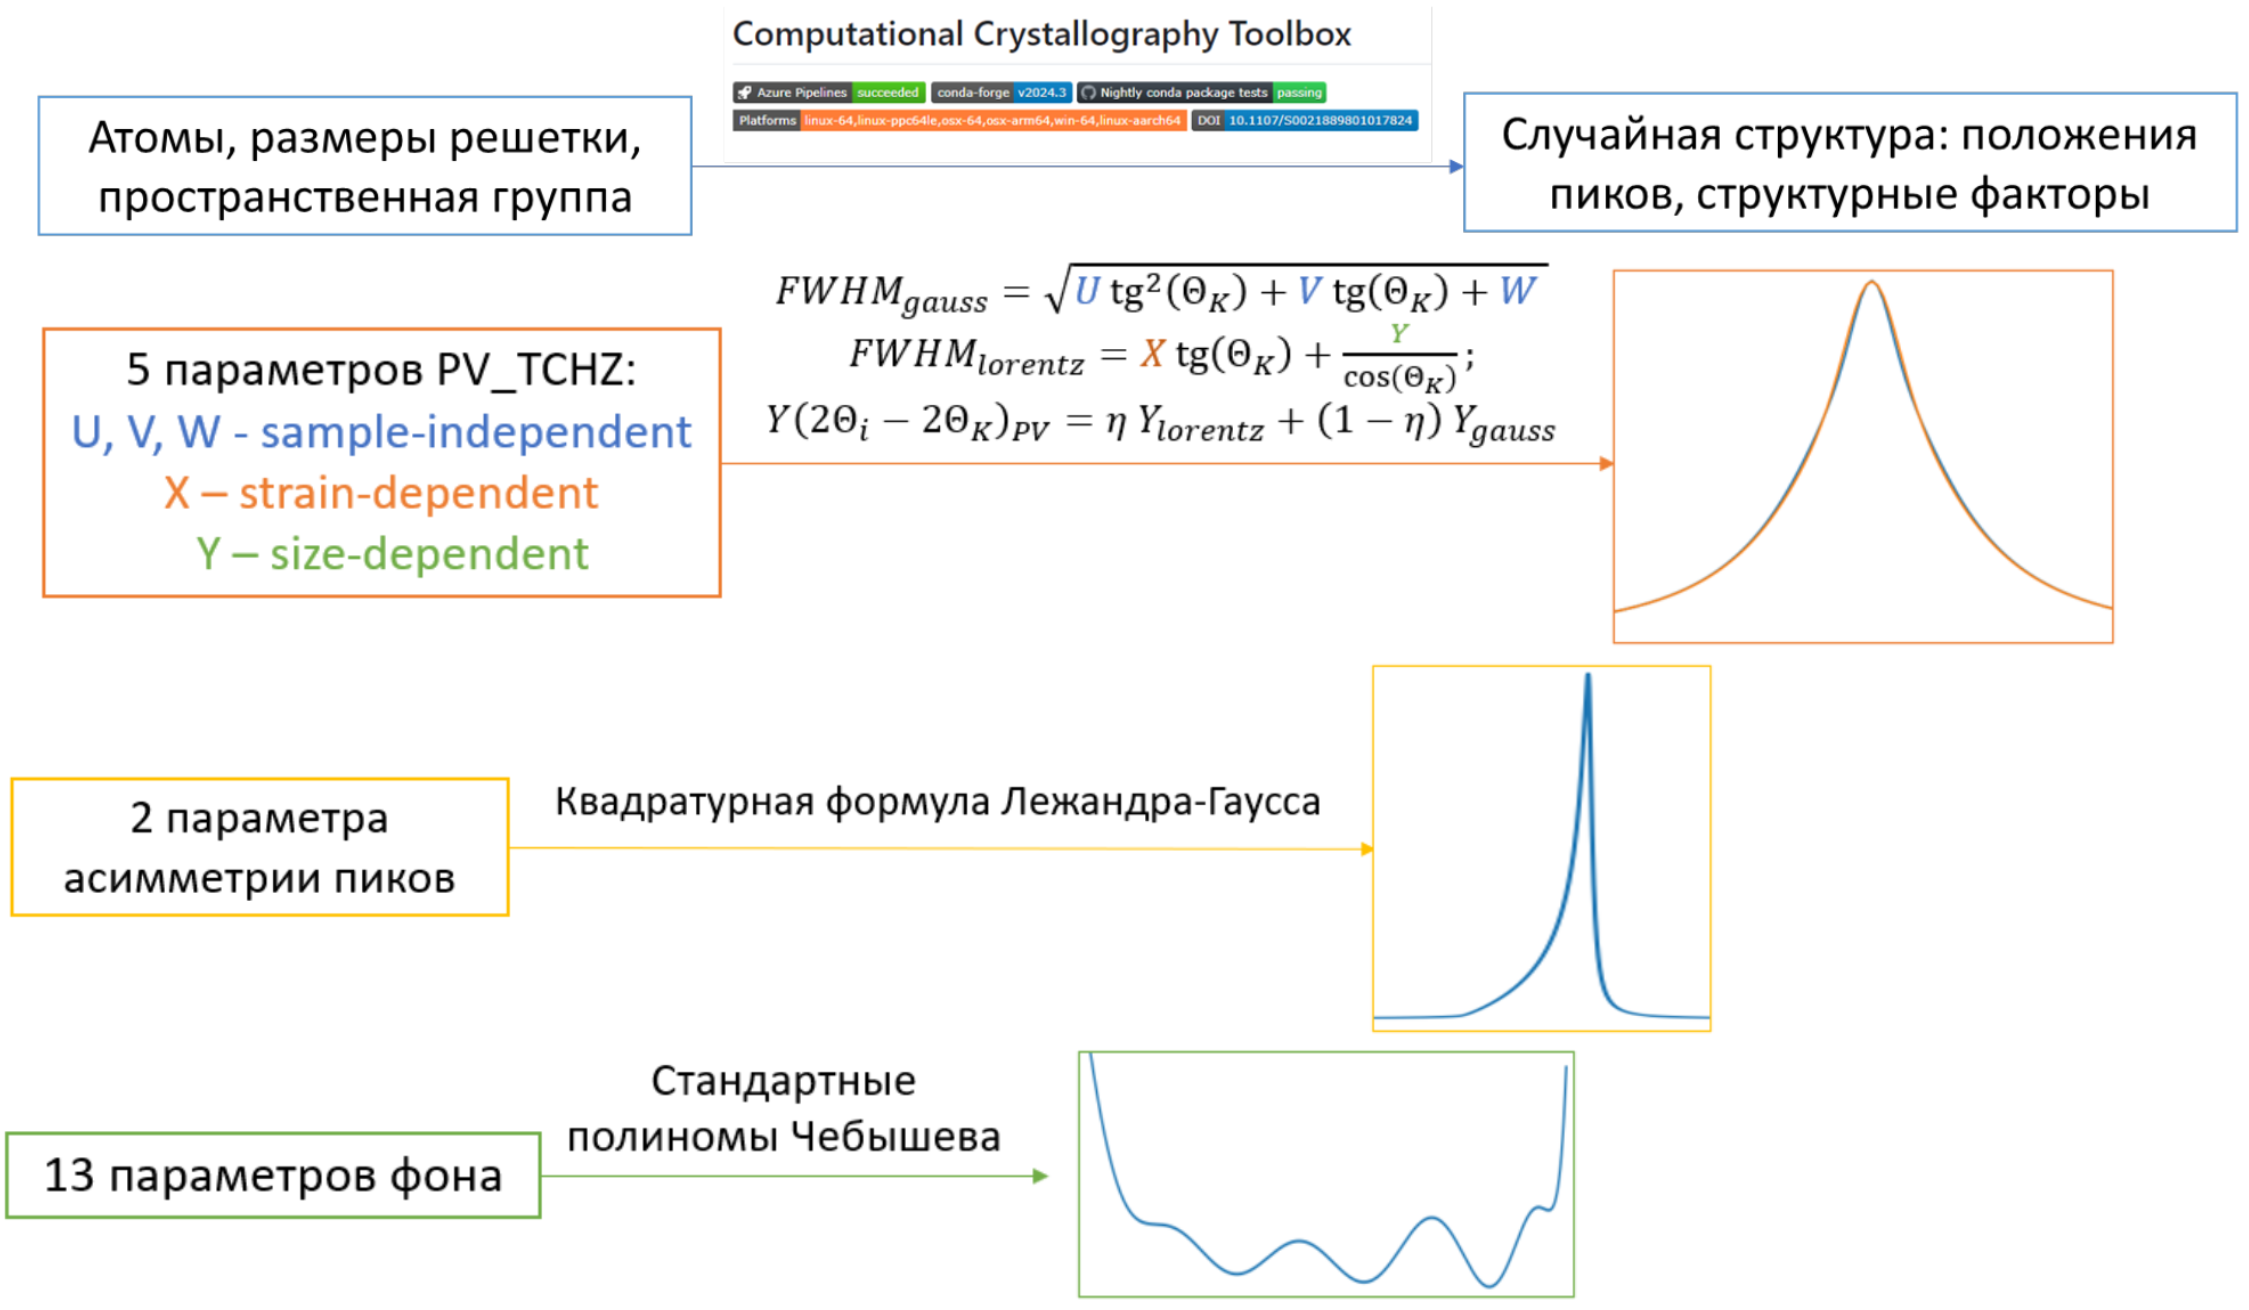
\includegraphics[width=1\textwidth]{figures/pxrd.png}\hfill
	\caption{Схема генерации случайных дифрактограмм в разработанной программе генерации}
	\label{pxrd}
\end{figure}

Начальное обучение моделей глубокого обучения было решено проводить на синтетических структурах, которые были получены с помощью созданного генератора. Так как общее количество симметрично независимых отражений зависит от класса Лауэ, было решено сосредоточиться на моноклинных структурах, поскольку моноклинные группы симметрии являются одними из наиболее распространенных для белковых структур в базе данных белков (\url{rcsb.org/stats/distribution-space-group}). При генерации структур её основные параметры (группа симметрии, типы атомов, их количество) определяются случайным образом (случайное сэмплирование) из следующих значений: 

\begin{itemize}
\item группы симметрии: P2$_1$, C2;
\item атомы: C, N, O, Cl, Br;
\item число симметрично независимых атомов в ячейке: 10--30;
\end{itemize}

При выполнении численных экспериментов со структурными факторами было решено работать с их амплитудами. Типичные распределения этих данных для сгенерированных структур представлены на рис. \ref{F_dist}. Как можно заметить, распределение амплитуд более пологое, чем интенсивностей, поэтому именно амплитуды были выбраны для решения задачи. 


\begin{figure}[H]
			\centering
            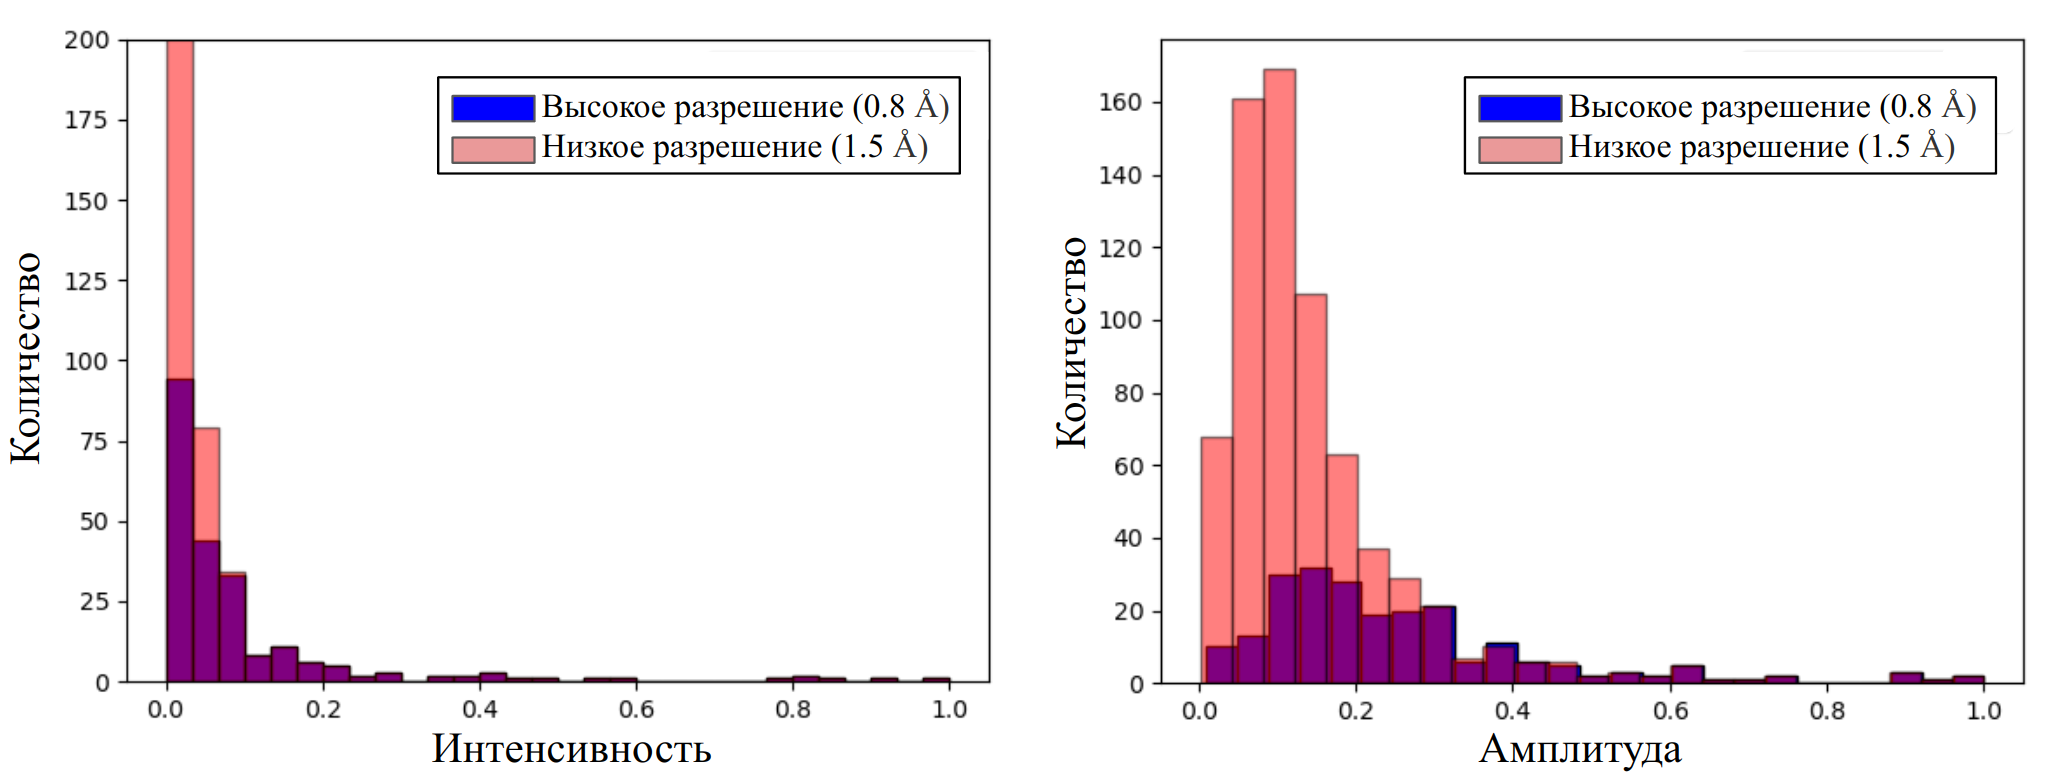
\includegraphics[width=1\textwidth]{figures/F_both.png}
            \caption{Типичные распределения интенсивностей (слева) и амплитуд (справа) дифракционной картины}
            \label{F_dist}
\end{figure}


600.000 полученных структур были разделены на наборы следующих размеров: 400.000, 100.000 и 100.000 для тренировочной, валидационной и тестовой выборок, соответственно. Из этих структур были собраны следующие наборы данных, с помощью которых будет проведено обучение моделей:

\begin{enumerate}
\item $D_1 = \left\lbrace\mathbf{F(1.5\angstrom)_{i}, F(0.8\angstrom)_{i}}\right\rbrace^n_{i=1}$

\item $D_2 = \left\lbrace\mathbf{F(1.2\angstrom)_{i}, F(1.0\angstrom)_{i}}\right\rbrace^n_{i=1}$

\item $D_3 = \left\lbrace\mathbf{E(1.2\angstrom)_{i}, E(1.0\angstrom)_{i}}\right\rbrace^n_{i=1}$

%\item $D_4 = \left\lbrace\mathbf{P_{1.5\angstrom, i}, F_{0.8\angstrom, i}}\right\rbrace^n_{i=1}$
\end{enumerate}

Также в работе использовались реальные моноклинные молекулярные структуры малых молекул из Кембриджского Банка Структурных Данных \cite{groom_cambridge_2014}, для которых были расчитаны дифракционные отражения. 10.000 структур использовались для дообучения моделей на реальных структурах, 2000~--- были отложены для тестирования. На рис. \ref{max_qty} представлена зависимость среднего количества отражений от выбранного разрешения дифракционной картины. При повышении разрешения с 1.5 \angstrom  до  0.8 \angstrom (набор $D_1$) требуется с помощью нейронной сети увеличить число максимумов более чем в 5 раз, поэтому был также собран набор $D_2$, для которого потребуется расширить дифракционную картину в 1.7 раз. 



\begin{figure}[H]
			\centering
            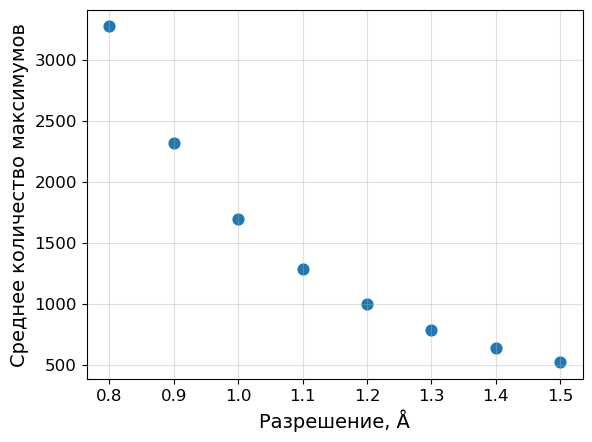
\includegraphics[width=0.8\textwidth]{figures/max_qty.png}
            \caption{Зависимость среднего количества дифракционных отражений моноклинных (P2$_1$, C2) структур из CSD от разрешения}
            \label{max_qty}
\end{figure}

Рассчитанный набор амплитуд нормализованных структурных факторов $D_3$ использован из соображения, что нормализованные структурные факторы $E$ лишены явной зависимости амплитуды от $\frac{\sin \theta}{\lambda}$, где $\Theta$~--- угол отражения, $\lambda$~--- длина волны рентгеновского излучения. Это приводит к тому, что распределение $|E|$ менее смещено в сторону высокоинтенсивных максимумов по сравнению
 с $|F|$ (рис. \ref{amplfehist}), что делает данный набор данных более перспективным для решения с помощью машинного обучения, поскольку требуется предсказывать низкоинтенсивные отражения.
 
\begin{figure}[H]
			\centering
            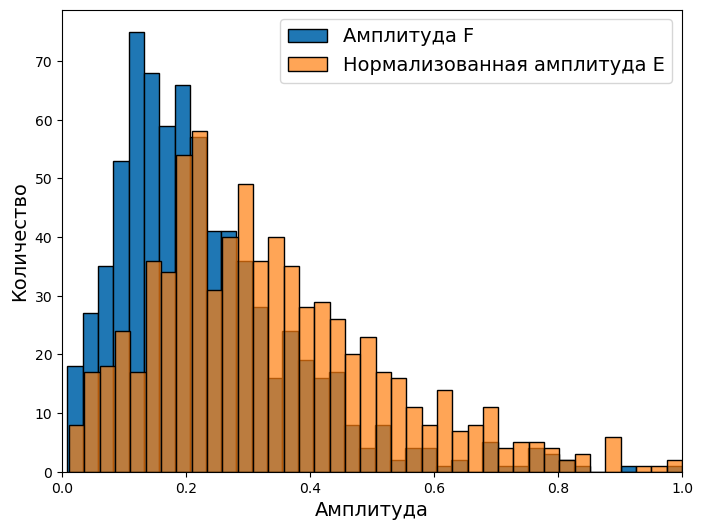
\includegraphics[width=0.8\textwidth]{figures/amplfehist.png}
            \caption{Типичные распределения амплитуд структурного фактора $F$ и нормализованного структурного фактора $E$ (разрешение 1.0 \angstrom)}
            \label{amplfehist}
\end{figure}

Размер полученных тензоров составляет (26, 18, 23) для набора данных $D_1$ и (23, 16, 21) для наборов $D_2$, $D_3$ --- в тензоры таких размерностей помещаются все отражения для самой большой моноклинной структуры из синтетических данных (для разрешения 0.8 \angstrom и 1.0 \angstrom). Также значения в каждом тензоре были отнормированы в диапазон 0--1.

 

\subsection{Модели машинного обучения}

Обозначим модель машинного обучения как $g(\mathbf{\Theta}, \mathbf{F})$, которая задаётся параметрами $\mathbf{\Theta}$ и принимает на вход тензор рентгенодифракционных отражений $\mathbf{F}$. Модель рассчитывает дополненный тензор отражений $\mathbf{F_{high}^g} = g(\mathbf{\Theta}, \mathbf{F_{low}})$, который должен быть максимально близок к реальной дифракционной картине высокого разрешения $\mathbf{F_{high}}$. Задача является регрессионной, процесс обучения на наборе данных, состоящего из пар $\left\lbrace\mathbf{F_{low, i}, F_{high, i}}\right\rbrace^n_{i=1}$ стремится оптимизировать параметры $\mathbf{\Theta}$, минимизируя целевую функцию, в качестве которой выбрана среднеквадратичная ошибка (MSE):

\begin{equation}
\mathrm{\mathbf{\Theta^*} = \argmin_{\mathbf{\Theta}} \left[ MSE(\mathbf{\Theta}) := \frac{1}{n}\sum\limits_{i=1}^n\|g(\mathbf{\Theta}, \mathbf{F_{low}}) - \mathbf{F_{high}}\|^2_F\right]}
\end{equation} 


Как уже было отмечено, в качестве функции потерь была выбрана среднеквадратичная ошибка, минимизация которой должна приводить к восстановлению тензора рентгеновских отражений. В качестве метрики для оценки эффективности моделей также был использован R-фактор:

\begin{equation}
\mathrm{R = \frac{\sum\limits_{h,k,l}|F_{obs}-F_{calc}|}{\sum\limits_{h,k,l}|F_{obs}|}},
\end{equation}

где $|F_{obs}|$~--- экспериментальные структурные факторы, $|F_{calc}|$~--- рассчитанные по модели структурные факторы. R-фактор является общепринятым стандартом в кристаллографическом сообществе для оценки качества структурных моделей. Нулевое значение R-фактора отвечает идеальному соответствию между данными модельной структуры и экспериментальными данными. В качестве экспериментальных структурных факторов в работе были использованы структурные факторы, рассчитанные по структуре, а $F_{calc}$~--- результат вычислений с помощью нейронных сетей.

Также в качестве метрики сравнения изображений рассматривался индекс структурного сходства SSIM \cite{zeng_3d-ssim_2012}, который зарекомендовал себя как хорошая метрика для оценки восстановления и увеличения разрешения изображений, однако эксперименты с ним в качестве добавки к функции потери привели к более низкому качеству восстановления модели с точки зрения R-фактора. Данный результат можно объяснить отсутствием локальной связанности наших данных.

В качестве базовой модели (baseline) была обучена модель UNet \cite{ronneberger_u-net_2015}, адаптированная для трехмерных данных (рис. \ref{unet}). Данная модель выбрана, потому что она хорошо себя проявляет в простейших задачах увеличения разрешения изображения за счет генерации недостающих пикселей на входных данных низкого разрешения (Super Resolution).

\begin{figure}[H]
    \centering
    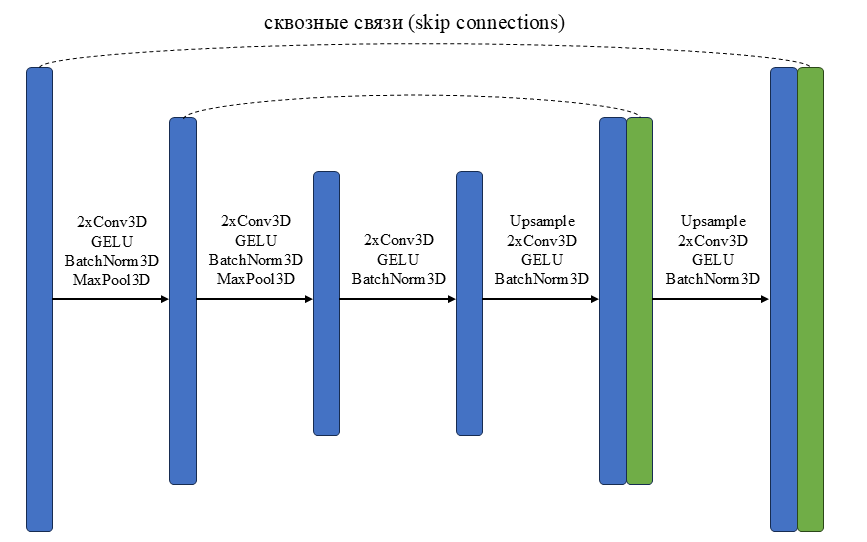
\includegraphics[width=0.8\textwidth]{figures/unet_arch.png}
    \caption{Схемы архитектуры модели UNet}
    \label{unet}
\end{figure}

Также была разработана и обучена модель на основе UNet с улучшенными слоями, содержащими Фурье-преобразование FFT\_UNet (рис. \ref{fft_unet}). Данный подход был продемонстрирован \cite{yang_hionet_2023} при работе с дифракционными данными и он является многообещающим и для нашей задачи, поскольку при переходе в прямое пространство наши данные являются локально связанными.


\begin{figure}[H]
    \centering
    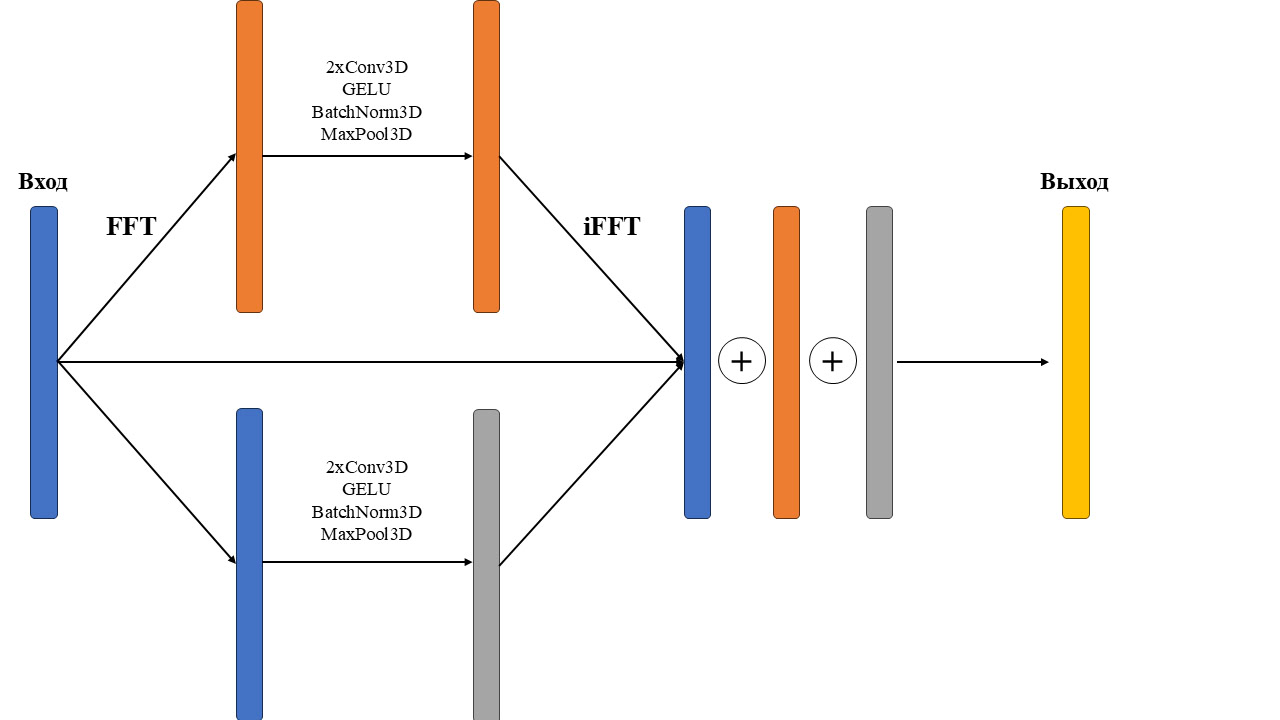
\includegraphics[width=1\textwidth]{figures/fft_arch.jpg}
    \caption{Схема слоёв с преобразованием Фурье}
    \label{fft_unet}
\end{figure}

Поскольку тензоры отражений не являются локально связанными, актуально использование механизма внимания. Он позволит модели находить связи между дальними отражениями. Так, был разработан трансформер XRD\_Transformer для нашей задачи (рис. \ref{XRDTrans}). 

\begin{figure}[H]
    \centering
    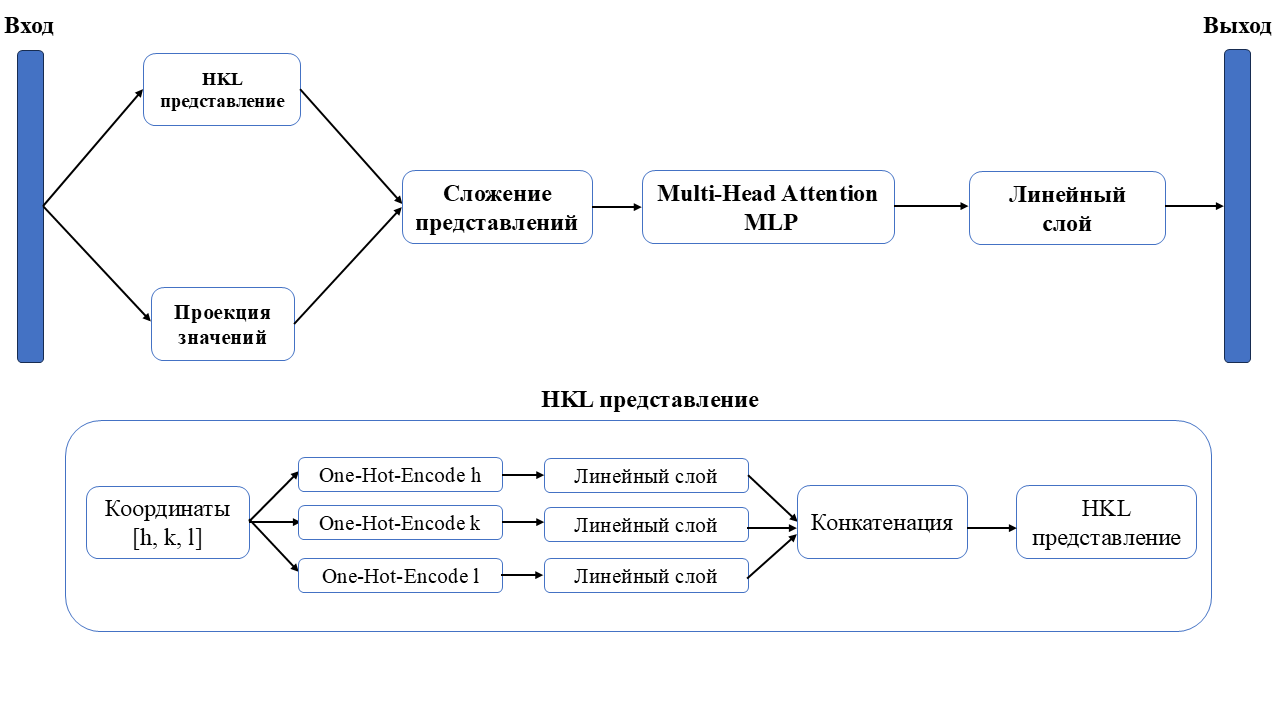
\includegraphics[width=1\textwidth]{figures/xrd_arch.png}
    \caption{Схема архитектуры XRD\_Transformer}
    \label{XRDTrans}
\end{figure}

В модели формируется единое векторное представление (embedding) из индексов Миллера и проекции значений амплитуды отражений, затем он проходит через 5 слоев трансформера, которые состоят из слоев многоголового внимания (Multi-Head Attention) и блоков многослойного перцептрона (MLP). Затем после нормализации (LayerNorm) и обратного проецирования в исходное пространство получается восстановленный тензор дифракционной картины.

Так как нам известны все возможные значения индексов Миллера (h, k, l) для структур выбранных размеров с заданным разрешением, HKL представления (рис. \ref{XRDTrans}) формируется следующим образом: индексы кодируются с помощью унитарного кодирования (One-Hot Encoding), после чего каждый вектор с помощью обучаемого линейного слоя проецируется в вектор размерности $\frac{embed\_dim}{3}$ после конкатенации размерность полученного векторного представления составляет $embed\_dim$. Также в модели реализована возможность получения представления через полносвязный слой, который проецирует позицию (h, k, l) сразу в вектор, однако она не использовалась при обучении модели, так как первый способ является более физическим для нашей задачи, поскольку мы используем только симметрически независимые отражения.


%\begin{figure}[H]
%    \centering
%    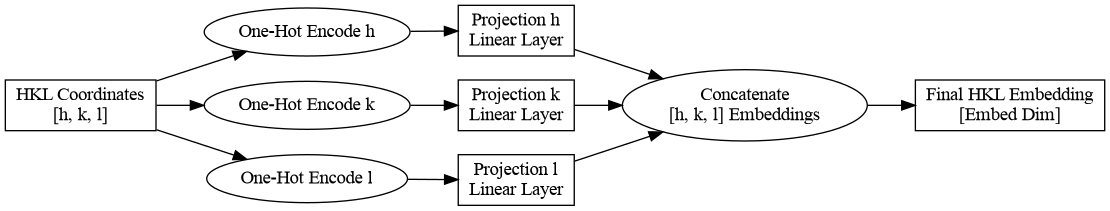
\includegraphics[width=1\textwidth]{figures/hkl_embedding_process.png}
%    \caption{Схема формирования эмбеддинга HKL}
%    \label{hklembed}
%\end{figure}


\section{Обсуждение результатов}

\subsection{Результаты обучения}

В рамках данной работы был разработан автоматизированный конвейер (пайплайн), позволяющий проводить воспроизводимые эксперименты по решению проблемы фаз с помощью предложенного метода (\url{github.com/blackwood168/xrd_phase_ml}). В нем реализовано обучение и тестирование моделей, а также получение результатов на реальных массивах данных и структурах кристаллических соединений. В репозитории присутствуют маленькие наборы данных из сгенерированных и реальных структур малых органических молекул, также там представлены веса обученных в работе моделей. Воспроизводимость обучения обеспечивает фиксирование начальных значений генераторов случайных состояний.

\begin{table}[H]
\caption{Результаты обучения и эффективность дообучения моделей}
\label{doposle}
\centering
\footnotesize
\begin{tabular}{|l|l|l|l|} 
\hline
\textbf{Model} & \textbf{Metric} & \textbf{Synth} & \textbf{CSD}  \\ 
\hline
\multirow{3}{*}{UNet} 
& Before, R & 0.477 & 0.590 \\ 
& After, R  & 0.632 & 0.393 \\ 
& $\Delta$, \%       & -32.6 & 33.4  \\
\hline
\multirow{3}{*}{FFT\_UNet}
& Before, R & 0.726 & 0.646 \\ 
& After, R  & 0.619 & \textbf{0.336} \\ 
& $\Delta$, \%       & 14.7  & 48.0  \\
\hline
\multirow{3}{*}{XRD\_Transformer}
& Before, R & 0.346 & 0.581 \\ 
& After, R  & 0.615 & 0.358 \\ 
& $\Delta$, \%       & -77.9 & 38.4  \\
\hline
\end{tabular}
\end{table}

Было проведено обучение на синтетических данных и последующее дообучение на реальных. Сравнение R-фактора для моделей до и после дообучения представлено в таблице \ref{doposle}. После дообучение на реальных данных точность предсказания моделей увеличивается минимум в 1.5 раза, однако теряют в точности на синтетических данных, кроме кастомного UNet с Фурье-преобразованием. Лучшую точность имеет модель UNet\_FFT, от которой немного отстает трансформер. В сводной таблице \ref{svod} представлены значения метрик на реальных данных финальных моделей. Таким образом, UNet\_FFT занимает меньше видеопамяти, работает быстрее и достигает лучшей метрики на тестовых реальных данных.

\begin{table}[H]
\centering
\caption{Значения метрик на тестовом реальном наборе данных моделей после дообучения}
\label{svod}
\begin{tabular}{|c|c|c|c|} 
\hline
\diagbox{\textbf{Metric}}{\textbf{Model}} & \textbf{UNet} & \textbf{FFT\_UNet} & \textbf{XRD\_Transformer}  \\ 
\hline
MSE$\cdot10^{-3}$                               & 1,39      & 1,20           & 1,31                   \\ 
\hline
R                                & 0,393         & \textbf{0,336}              & 0,358                      \\
\hline
\end{tabular}
\end{table}

\subsection{Анализ моделей}

Для более глубокого понимания трансформера был проведен анализ внутренней работы модели. Особый интерес представляют карты внимания (рис. \ref{attention_maps}), которые визуализируют, как модель распределяет свое внимание при обработке дифракционных данных тестовой реальной кристаллической структуры. Механизм внимания в трансформере позволяет модели определять, какие части входных данных наиболее важны для принятия решения в каждый момент времени. В первых слоях трансформера внимание распределено равномерно и рассеянно по всей структуре данных. Это соответствует этапу сбора общего контекста, когда модель пытается получить целостное представление о кристаллической структуре. В последующих слоях внимание становится более сфокусированным и локализованным, что указывает на то, что модель научилась выделять специфические взаимосвязи между различными частями данных. Важно отметить способность модели устанавливать связи между отражениями, находящимися на значительном расстоянии друг от друга в обратном пространстве. Это критически важно для решения проблемы фаз, так как часто ключевые взаимосвязи существуют между отражениями, которые не являются ближайшими соседями. Кроме того, наблюдаются характерные диагональные паттерны внимания, которые коррелируют с известными систематическими погасаниями в кристаллографии. Можно предположить, что модель глубокого обучения без явного указания из обучающей выборки выучила механизм погасаний.

\begin{figure}[H]
    \centering
    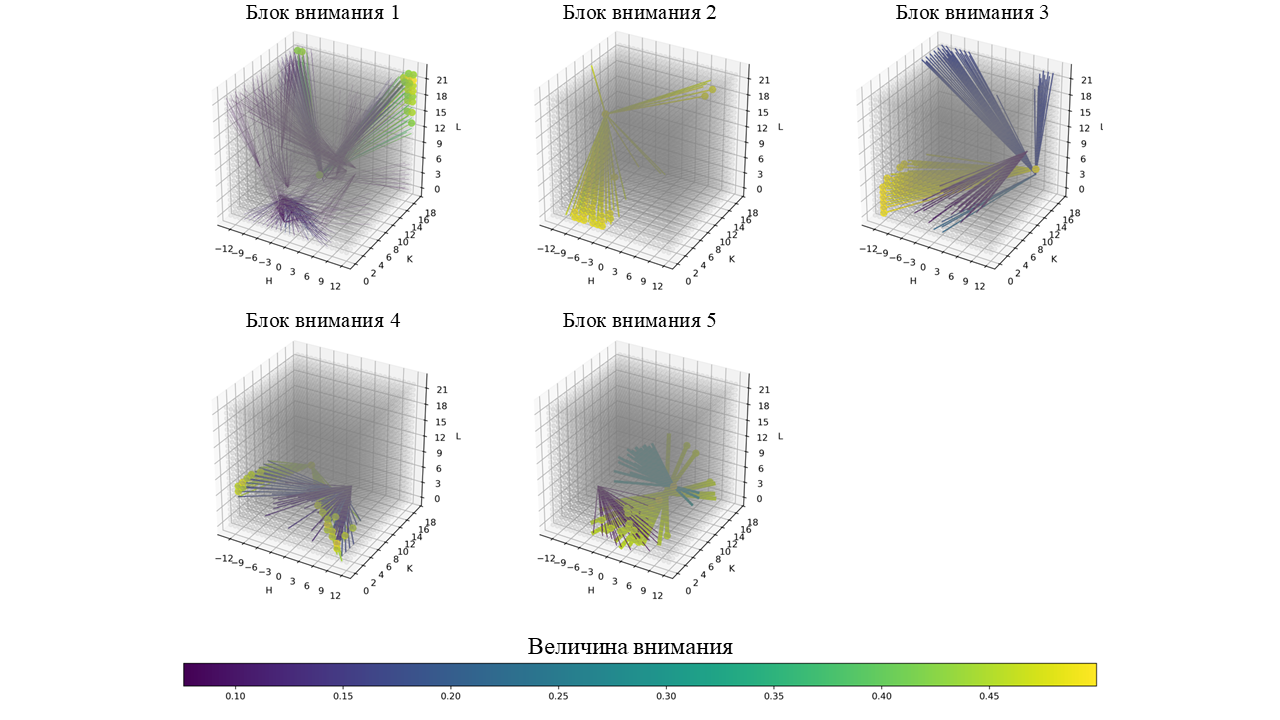
\includegraphics[width=1\textwidth]{figures/attention.png}
    \caption{Связи внимания в блоках трансформера}
    \label{attention_maps}
\end{figure}

Для количественного подтверждения этой гипотезы, было проанализировано распределение значений внимания для наиболее сильных связей в каждом блоке трансформера (рис. \ref{att_hist}). Особый интерес представляет сравнение двух типов связей: между точками, соответствующим систематическим погасаниям и обычными отражениями. Можно заметить, что во время сбора общего контекста в первом блоке распределение значений внимания для связей с погасшими отражениями сопоставимо с таковым для обычных отражений. Это логично, поскольку на этом этапе модель еще не дифференцирует типы отражений, а просто собирает общую информацию о структуре. Однако уже во втором блоке наблюдается значительно уменьшение связей внимания, соединяющих погасания. Это указывает на то, что модель начинает осознавать, что эти отражения несут меньше полезной информации, требуемой для предсказывания дальних отражений. В третьем же блоке модель игнорирует точки обратного пространства, соответствующие систематическим погасаниям, и в выходном тензоре на соответствующих местах стоят нули. 

\begin{figure}[H]
    \centering
    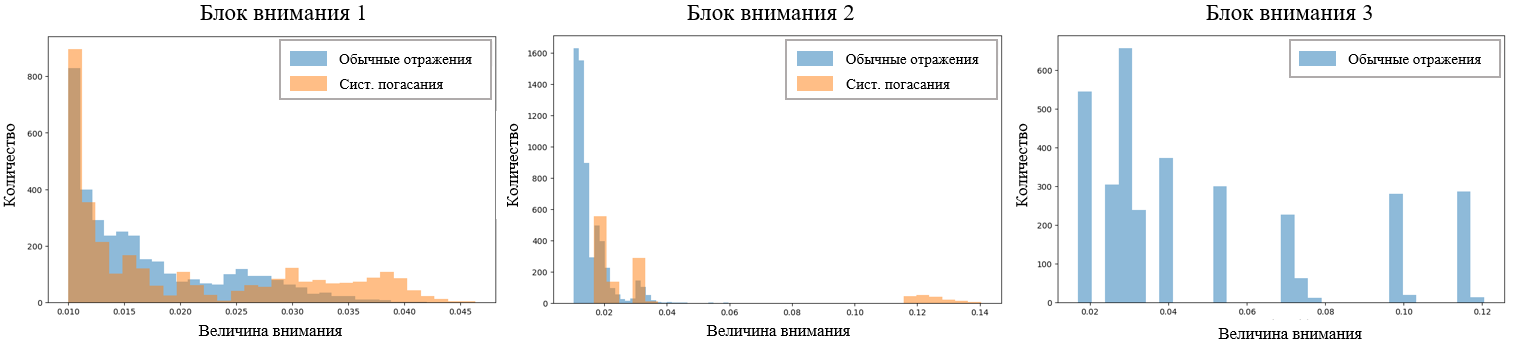
\includegraphics[width=1\textwidth]{figures/attention_hist.png}
    \caption{Распределение величин внимания в первых блоках трансформера.}
    \label{attention_maps}
\end{figure}

Такое поведение модели демонстрирует, что она не просто запомнила шаблоны из обучающей выборки, а научилась автоматически определять и игнорировать отражения, соответствующие систематическим погасаниям (если такие присутствуют). Трансформер действительно успешно выучил кристаллографическую закономерность, значит, данная архитектура может являться ключевой для дальнейших исследований применения методов глубокого обучения для решений кристаллографических задач.

Для понимания внутренней работы моделей на основе UNet, был проведен анализ первого блока обеих архитектур с помощью метода GradCAM (рис. \ref{gradcam}) \cite{selvaraju_grad-cam_2020}. Этот метод позволяет визуализировать, какие области входных данных имеют наибольшее влияние для принятия решений моделью.


\begin{figure}[H]
     \centering
     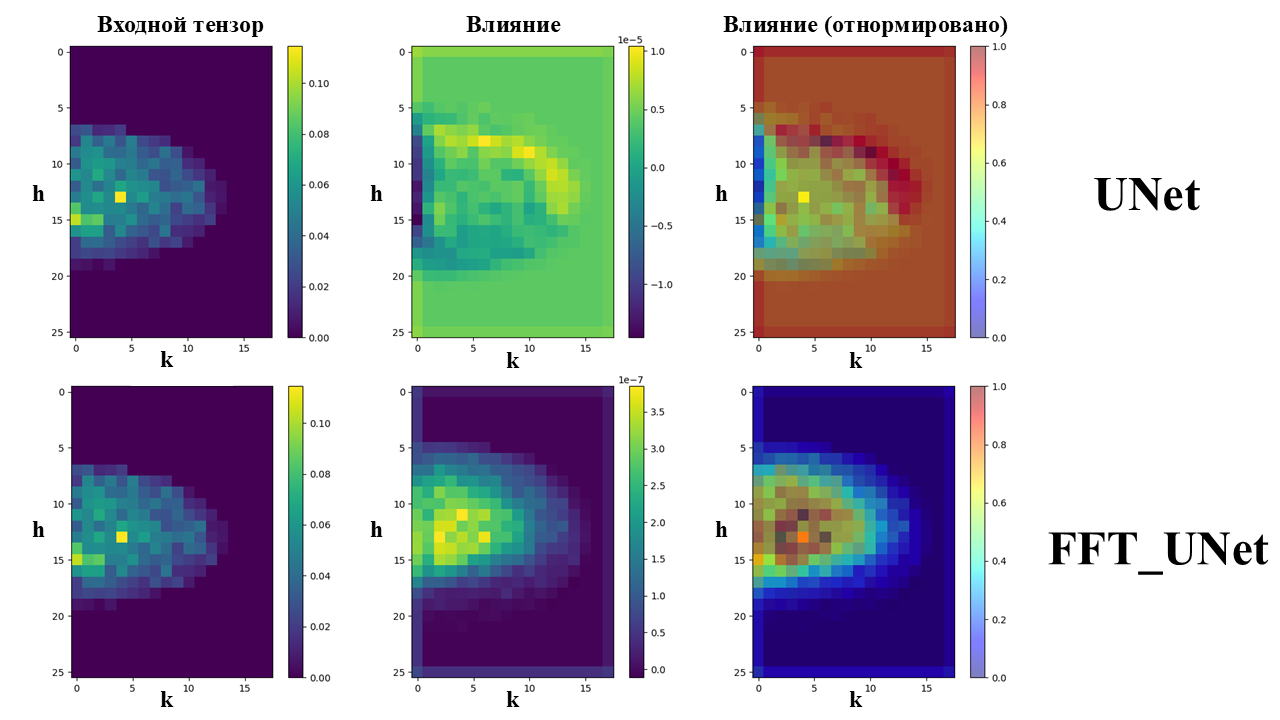
\includegraphics[width=1\textwidth]{figures/attribute_map.png}
     \caption{Тепловые карты влияния GradCAM}
     \label{gradcam}
\end{figure}

%\begin{figure}[H]
%    \centering
%    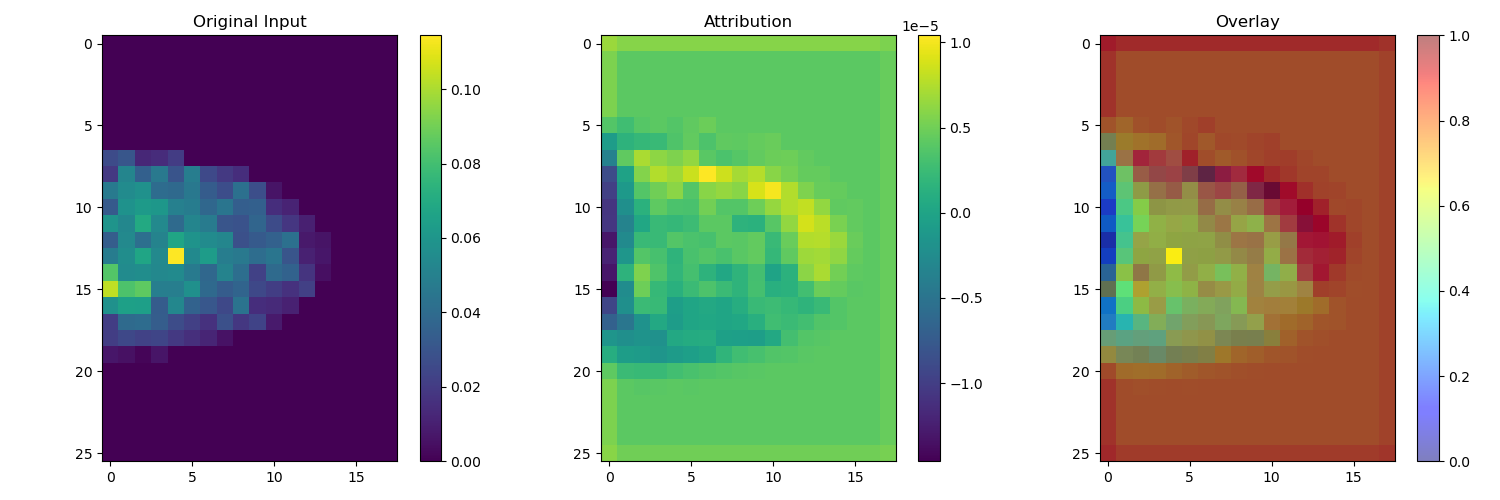
\includegraphics[width=1\textwidth]{figures/attribution_overlay.png}
%    \caption{Анализ первого блока UNet с помощью GradCAM}
%    \label{gradU}
%\end{figure}
%
%\begin{figure}[H]
%    \centering
%    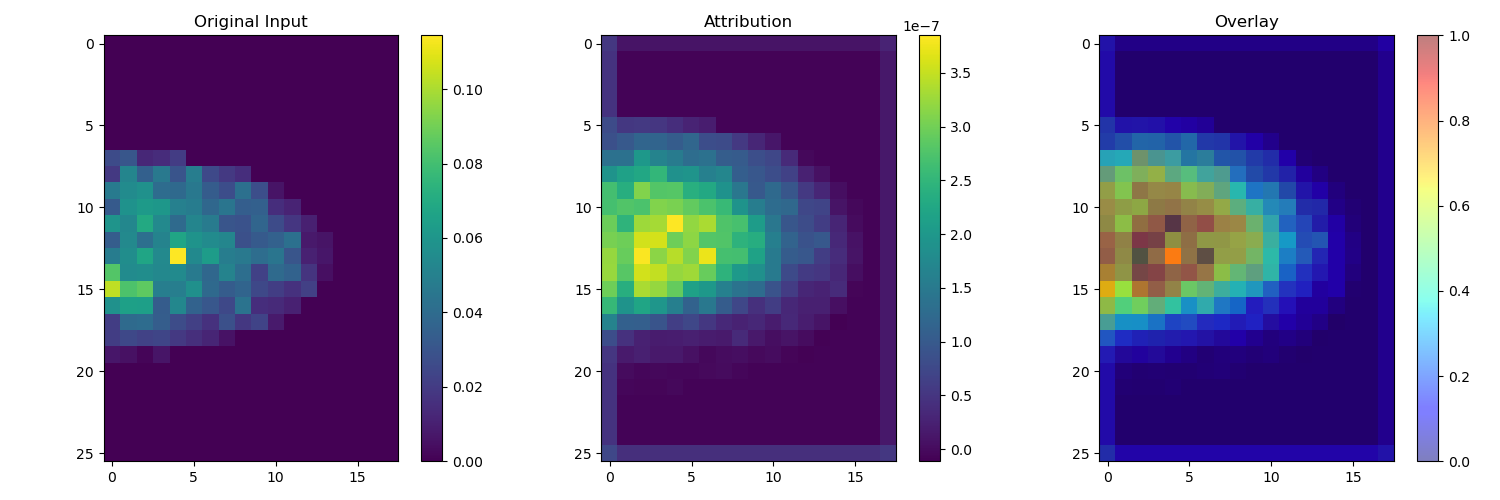
\includegraphics[width=1\textwidth]{figures/attribution_overlay_fft.png}
%    \caption{Анализ первого блока FFT\_UNet с помощью GradCAM}
%    \label{gradFFT}
%\end{figure}

Анализ тепловой карты влияния для модели UNet показал интересную особенность: модель концентрируется во всем пространстве за пределами изначальной дифракционной картины низкого разрешения. Это может указывать на то, что модель UNet не полностью учитывает физические ограничения задачи и пытается извлечь информацию из областей, где она физически не может существовать. 

В отличие от UNet, паттерн внимания для FFT\_UNet выглядит более физически обоснованным. Значения влияния распространяются преимущественно на область входной дифракционной картины и немного выходят за её границы. Это поведение более физически обосновано, так как модель ищет информацию вблизи границ дифракционной картины, где могут находиться важные детали структуры. 

Это различие в поведении моделей может объяснять, почему FFT\_UNet показывает лучшие результаты в восстановлении дифракционной картины. Её способность более точно определять области, где может находиться полезная информация, и игнорировать физически нереалистичные области, делает её более эффективной в поиске правильного решения.



\begin{figure}[H]
    \centering
    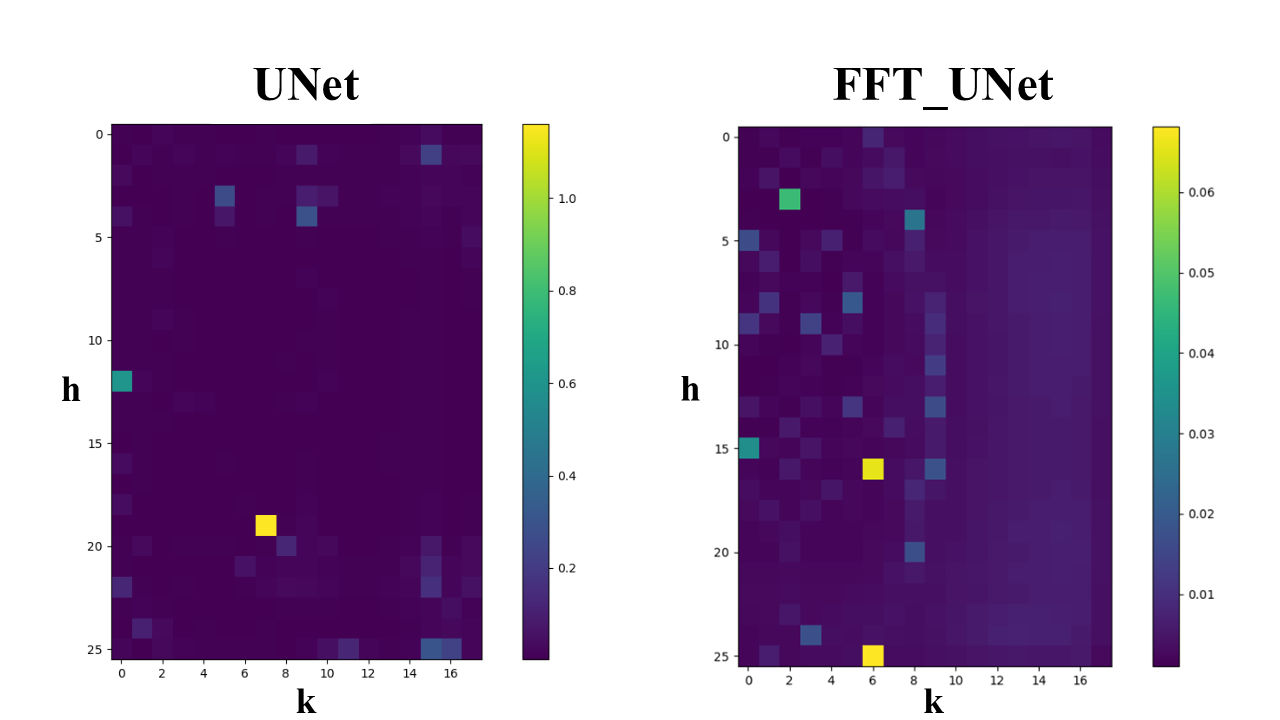
\includegraphics[width=1\textwidth]{figures/sensitivity.png}
    \caption{Тепловые карты чувствительности}
    \label{sens}
\end{figure}


Для оценки устойчивости моделей к шуму в экспериментальных данных был проведен анализ карт чувствительности (рис. \ref{sens}). Карты чувствительности показывают, как сильно меняется выход модели при добавлении случайного шума к входным данным, что позволяет оценить устойчивость модели в различных областях обратного пространства. Базовая модель UNet демонстрирует неустойчивое поведение – выход модели может измениться при добавлении шума на очень большие значения. Модель с Фурье-преобразованием FFT\_UNet стабильно работает при наличии шума в данных. Высокая робастность в большей части пространства указывает на то, что модель научилась извлекать надежные признаки из данных и не переобучилась на конкретные значения амплитуд структурных факторов. 


\subsection{Проверка на реальных данных}

Хотя модели демонстрируют обнадеживающие результаты на реальных моноклинных структурах из Кембриджского Банка Структурных данных, качество восстановления тензора отражений все еще недостаточно для решения структуры с помощью программы SHELXT. На рис. \ref{recon_ex} представлены характерные сечения тензора отражений для реальной структуры, где R-фактор восстановленного тензора с помощью FFT\_UNet составляет 0.35.

\begin{figure}[H]
    \centering
    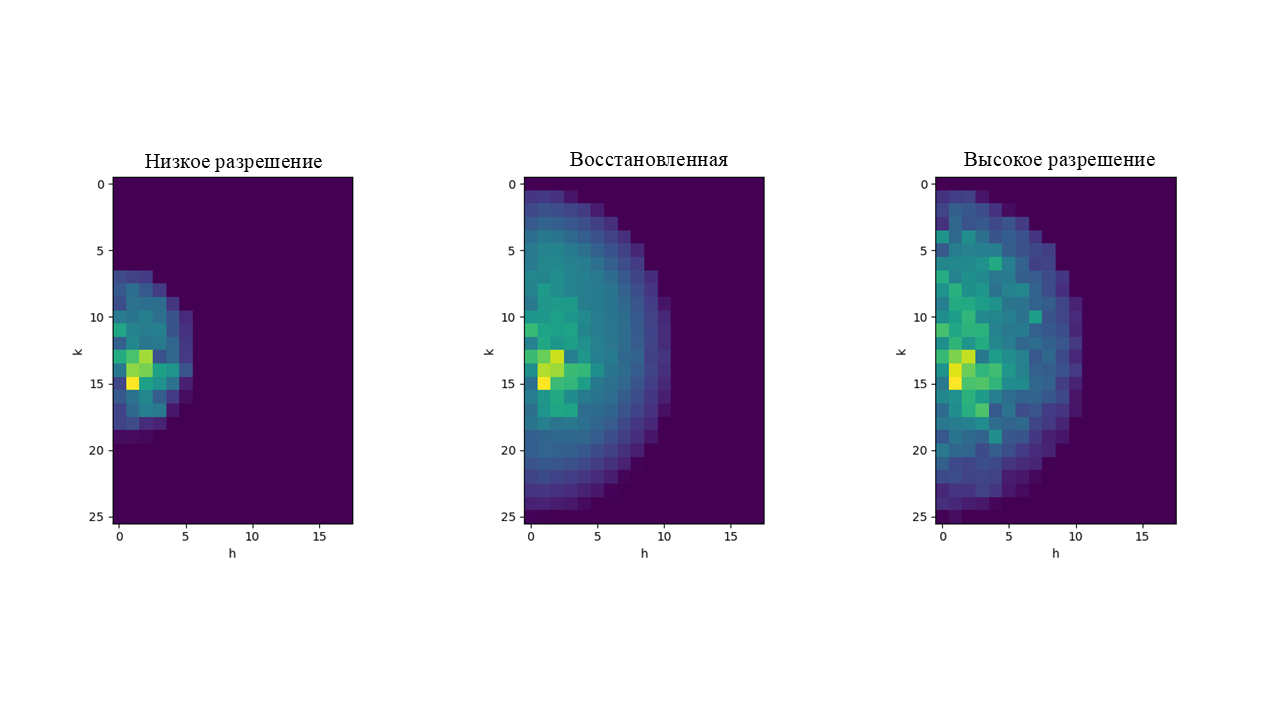
\includegraphics[width=1\textwidth]{figures/real.png}
    \caption{Типичная реконструкция дифракции реальной структуры, $R = 0.346$}
    \label{recon_ex}
\end{figure}

Анализ результатов показывает, что нейронная сеть успешно справляется с определением общих характеристик дифракционной картины. Она точно предсказывает границы дифракционной картины и корректно восстанавливает средние значения амплитуд структурных факторов по небольшим областям. Однако изменения амплитуд между соседними точками обратного пространства недостаточно четко выражены, что приводит к потере важных деталей в распределении амплитуд. 

Это ограничение становится особенно критичным, если учесть фундаментальную особенность дифракционных отражений: каждое отражение содержит информацию о всей кристаллической структуре, и для успешного решения проблемы фаз необходимо чрезвычайно точное определение амплитуды в каждой точке. Хотя модели глубокого обучения выявляют некоторые кристаллографические закономерности, они не достигают необходимой точности в численном определении значений для каждой точки.

Таким образом, методы глубокого обучения демонстрируют значительный потенциал в распознавании кристаллографических закономерностей в обратном пространстве, но сталкиваются с фундаментальным ограничением при решении проблемы фаз. Это ограничение связано с необходимостью чрезвычайно точного численного восстановления амплитуд отражений, что требует более точного подхода к определению значений в каждой точке. Это наблюдение указывает на необходимость разработки новых архитектур или подходов, которые могли бы сочетать способность к распознаванию паттернов с более точным численным восстановлением.

\subsection{Дальнейшие планы и предложения}

Было показано, что методы глубокого обучения успешно схватывают кристаллографические закономерности, однако из-за специфики обратного пространства для решения проблемы фаз им не хватает точности. Совершив переход в прямое пространство, можно предположить, что нейронные сети справятся с поставленной задачей.

Для решения проблемы фаз часто используется функция Паттерсона:

\begin{center}
    $P(u, v, w) = \sum\limits_{h,k,l\in Z} |F(h,k,l)|^2e^{-2\pi i(hu+kv+lw)}$
\end{center}

Функция Паттерсона является Фурье-преобразованием интенсивностей дифракционных максимумов, где за их фазы приняты нули. Таким образом, перейдя от тензора отражений к карте функции Паттерсона - получается классическая задача повышения разрешения изображений, поскольку для дифракционной картины низкого разрешения получится Фурье-образ низкого разрешения, разрешение которого требуется повысить так, чтобы восстановленная картина соответствовала Фурье-образу дифракционной картины высокого разрешения. После увеличения разрешения трехмерной картины функции Паттерсона, мы можем вернуться в обратное пространство, рассчитав интенсивности (и из них амплитуды) рентгенодифракционных отражений, и решить проблему фаз с помощью уже существующих ab initio методов.

\begin{figure}[H]
    \centering
    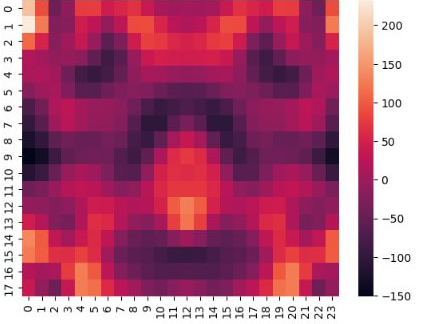
\includegraphics[width=0.5\textwidth]{figures/patt_high.png}\hfill
    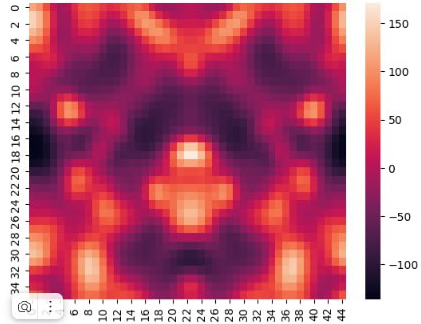
\includegraphics[width=0.5\textwidth]{figures/patt_low.png}
    \caption{Типичное сечение функции Паттерсона по данным низкого (слева) и высокого (справа) разрешения}
    \label{patt}
\end{figure}
%\newpage
\section{Заключение}
\sloppy{
Результаты данной работы показывают, что радиационная стойкость бензола, наблюдаемая в конденсированных средах, не определяется непосредственно молекулярными свойствами бензола, а является, в первую очередь, следствием эффективной диссипации энергии в конденсированных средах за счёт образования эксимеров бензола. Показано, что изолированные  молекулы бензола достаточно эффективно разлагаются в результате радиолиза в аргоновой матрице: в этих условиях значения радиационно-химических выходов разложения бензола в матрицах сопоставимы с выходами разложения других органических молекул в инертных матрицах. При этом характеристики матрицы (в частности, поляризуемость) оказывают большое влияние на радиационно-химический выход разложения бензола: в матрице аргона бензол расходуется при облучении примерно в 6 раз эффективнее, чем в более тяжёлых матрицах (Kr, Xe).

Показано, что основными каналами радиационно-индуцированных превращений бензола в матрицах инертных газов являются распад на фенильный радикал и атом водорода, а также изомеризация в фульвен. Характеристики матрицы (поляризуемость, атомный номер) существенно влияют на соотношение этих каналов. Отношение выходов фенильного радикала и фульвена резко возрастает в ряду Ar<Kr<Xe. Кроме того, зафиксировано образование {\itshape цис}- и {\itshape транс}-гексадиен\nobreakdash-1,3\nobreakdash-ина\nobreakdash-5, которые, вероятно, возникают в результате превращений возбуждённых молекул фульвена. Анализ дозовых зависимостей (кривых накопления) этих изомеров в различных матрицах показывает, что они могут возникать как непосредственно из бензола (без промежуточной стабилизации фульвена, образующегося предположительно в возбуждённом состоянии), так и в результате вторичного распада молекул фульвена, стабилизированных в матрицах.   

Впервые исследован радиолиз и фотолиз C$_6$D$_6$ в матрицах инертных газов. Показано, что дейтерирование не оказывает принципиального влияния на основные каналы радиолиза бензола и их соотношение. Основные тенденции, возникающие при радиолизе C$_6$H$_6$, сохраняются и в случае C$_6$D$_6$. Отсутствие влияния дейтерирования на основные каналы радиолиза, по-видимому, говорит о сравнительно малом вкладе процессов, протекающих через колебательно возбуждённые состояния, в образование основных первичных продуктов.   Впервые получены ИК-спектроскопические характеристики дейтерированных изомеров бензола (фульвена-$d_6$, бензвалена-$d_6$, бензола Дьюара-$d_6$).

Образующийся при радиолизе фенильный радикал является одним из ключевых интермедиатов  в предполагаемых механизмах образования ПАУ в космическом пространстве. Демонстрация эффективного образования этого радикала при радиолизе бензола (в отличие от фотолиза) в низкотемпературных матрицах может служить первым шагом на пути к экспериментальной верификации данных механизмов. Следует отметить, что состав продуктов при фотолизе и радиолизе бензола в матрицах различен из-за принципиально различных механизмов передачи энергии. Это обстоятельство необходимо учитывать при построении и верификации механизмов «холодного» синтеза ПАУ в межзвёздной среде.

В целом, сравнительное исследование механизмов радиационно-индуцированных превращений изолированных молекул бензола и его изотопологов при рентгеновском облучении в различных низкотемпературных инертных матрицах с использованием метода ИК-спектроскопии,  проведённое в данной работе, позволило получить принципиально новую информацию, которая может быть важна не только для астрохимии, но и для фундаментальной радиационной химии, фотохимии и спектроскопии.

}
\section{Заключение}

В данной работе представлен комплексный подход к решению проблемы фаз в рентгеновской кристаллографии с использованием методов глубокого обучения. Разработанное программное обеспечение для генерации синтетических рентгенодифракционных данных (\url{github.com/blackwood168/xrd_simulator}) создает надежную основу для обучения и тестирования моделей машинного обучения. Этот инструмент позволяет генерировать реалистичные дифракционные картины с учетом физических закономерностей, что критически важно для создания качественного обучающего набора данных.

Для обеспечения воспроизводимости экспериментов и стандартизации процесса разработки был создан единый конвейер (\url{github.com/blackwood168/xrd_phase_ml}), который включает в себя все этапы работы с данными: от их подготовки до обучения моделей и оценки их эффективности. Это значительно упрощает процесс разработки и позволяет сравнивать различные архитектуры на единой основе.

В рамках исследования были разработаны и протестированы три различные архитектуры нейронных сетей. В качестве базовой модели использовалась UNet, которая послужила отправной точкой для сравнения. FFT\_UNet, модифицированная версия UNet с встроенным преобразованием Фурье в слоях, была разработана с учетом специфики дифракционных данных. Особый интерес представляет XRD\_Transformer, архитектура на основе трансформера со специальным векторным представлением, который учитывает физические особенности задачи фаз. Все модели были обучены как на синтетических, так и на реальных кристаллических структурах, что позволило оценить их способность к обобщению.
Проведенный анализ внутренней работы моделей с использованием методов интерпретируемого ИИ (GradCAM, карты внимания, анализ чувствительности) подтвердил, что модели действительно выявляют некоторые фундаментальные кристаллографические закономерности. 

Текущие модели пока не достигают необходимого качества численного восстановления рентгеновских отражений для практического решения проблемы фаз. Это ограничение может быть связано с недостаточным учетом физических ограничений в архитектуре моделей и возможным несоответствием функции потерь физическим требованиям задачи. Для преодоления этих ограничений предлагается комплексный план изменений в подходе, включающий модификацию архитектуры моделей для лучшего учета физических ограничений, разработку специализированных функций потерь, учитывающих специфику проблемы фаз, и улучшение процесса обучения с использованием физически обоснованных ограничений

\section{Выводы}

\begin{itemize}
\item Разработано программное обеспечение по генерации синтетических рентгенодифракционных данных, которое может быть использование для решения прикладных задач рентгеновской дифракции с помощью ИИ (\url{github.com/blackwood168/xrd_simulator})

\item Разработан единый пайплайн (\url{github.com/blackwood168/xrd_phase_ml}), позволяющий проводить воспроизводимые эксперименты по обучению, тестированию и inference задачи предсказывания дальних отражений по ближним для решения проблемы фаз

\item Разработаны и обучены на синтетических и реальных структурах UNet в качестве baseline, FFT\_UNet --- кастомный UNet с Фурье-преобразованием в слоях, XRD\_Transformer --- модель на основе трансформер со специфичным эмбеддингом, вписывающимся в физику задачи

\item Проведен анализ моделей, подтверждающий, что модели глубокого обучения выявляют кристаллографические закономерности и имеют потенциал решения прикладных задач рентгеновской дифракции

\item У моделей не достает качества численного восстановления рентгеновских отражений для решения проблемы фаз, несмотря на улавливание рентгенодифракционных паттернов; приведено обоснование и предложен план изменения методологии для решения задачи

\end{itemize}



\newpage
\sloppy{
\addcontentsline{toc}{section}{Список литературы}
%\bibliographystyle{gost71s}
%\bibliographystyle{utf8gost705u}
%\bibliographystyle{utf8gost71s}
%\bibliographystyle{gost2008}
\bibliographystyle{gost2008l}
\bibliography{lit}
%\section*{Приложение}
\begin{center}
Приложение 1. Общий вид скрипта для генерации структурных данных
\end{center}
\begin{minted}[
frame=lines,
framesep=1.5mm,
baselinestretch=1.2,
bgcolor=LightGray,
fontsize=\footnotesize,
linenos
]{python}
SPACE_GROUPS = ['P21', 'C2']       
ELEMENTS = ["C", "N", "O", "Cl", "Br"]
N_ATOMS_LIMS = (10, 30)
ATOM_VOLUME_START_WIDTH = (14, 8)
d_high = 1.0  # High resolution limit
d_low = 1.2   # Low resolution limit
n_atoms = sample_gen(range(*N_ATOMS_LIMS))

# Initialize structure generator
str_generator = GenBuilder(
    classname=core.CctbxStr.generate_packing,
    sg=sample_gen(SPACE_GROUPS),
    atoms=sample_gen(ELEMENTS, size=n_atoms),
    atom_volume=distr_gen(sts.uniform(*ATOM_VOLUME_START_WIDTH)),
    seed=utils.distr_gen(sts.randint(1, 2**32-1))
)
def runner(pattern):
    """Process a single crystal structure pattern.
    Args:
        pattern: Crystal structure pattern object
    Returns:
        dict: Contains structure parameters and intensity data
    """
    ### Здесь разный код в зависимости от задачи ###
    
# Processing parameters
CHANKS = 50
CHANK_SIZE = 10000
CORES = 12
# Process structures in chunks
for i in range(CHANKS):
    chank = it.islice(str_generator, CHANK_SIZE)
    pool = mp.Pool(CORES)   
    with pool as p: results = p.map(runner, chank)
    directory = f'...'
    if not os.path.exists(directory): os.makedirs(directory)
    # Save results
    np.savez_compressed(f'{directory}/{i}',
        db=np.array(results)
    )
    pool.close()        
\end{minted}
\newpage

\begin{center}
Приложение 2. Функция runner для расчета интенсивностей случайных структур
\end{center}
\begin{minted}[
frame=lines,
framesep=1.5mm,
baselinestretch=1.2,
bgcolor=LightGray,
fontsize=\footnotesize,
linenos
]{python}
def runner(pattern):
    """Process a single crystal structure pattern.
    
    Args:
        pattern: Crystal structure pattern object
        
    Returns:
        dict: Contains structure parameters and intensity data
    """
    params = pattern.report_params()
    structure = pattern.structure
    
    # Calculate structure factors and intensities
    a_high = structure.structure_factors(d_min=d_high).f_calc().sort()
    I_high = a_high.as_intensity_array().data().as_numpy_array()
    ind_high = np.array(list(a_high.indices()))
    
    a_low = structure.structure_factors(d_min=d_low).f_calc().sort()
    ind_low = np.array(list(a_low.indices()))
    
    return {
        'structure_params': params,
        'ind_low': ind_low,
        'I_high': I_high,
        'ind_high': ind_high
    }
\end{minted}
\newpage

\begin{center}
Приложение 3. Функция runner для расчета нормализованных структурных факторов случайных структур
\end{center}
\begin{minted}[
frame=lines,
framesep=1.5mm,
baselinestretch=1.2,
bgcolor=LightGray,
fontsize=\footnotesize,
linenos
]{python}
def runner(pattern):
    """Process a single crystal structure pattern.
    
    Args:
        pattern: Crystal structure pattern object
        
    Returns:
        dict: Contains structure parameters and intensity data
    """
    params = pattern.report_params()
    structure = pattern.structure
    
    # Calculate structure factors and intensities
    a_high = structure.structure_factors(d_min=d_high).f_calc().sort()
    elements_to_parse = ['N', 'O', 'C', 'Cl', 'Br']
    asu_content = {}
    for scatterer in structure.scatterers():
        for elem in elements_to_parse:
            if scatterer.label == elem or scatterer.label.startswith(elem):
                asu_content[elem] = asu_content.get(elem, 0) + 1
    I_high = structure.structure_factors(d_min=d_high).f_calc().sort().as_intensity_array()
    e_high = a_high.as_amplitude_array().normalised_amplitudes(asu_content).array().data()
    e_high = e_high.as_numpy_array()
    ind_high = np.array(list(a_high.indices()))
    
    a_low = structure.structure_factors(d_min=d_low).f_calc().sort()
    e_low = a_low.as_amplitude_array().normalised_amplitudes(asu_content).array().data()
    e_low = e_low.as_numpy_array()
    ind_low = np.array(list(a_low.indices()))
    
    return {
        'structure_params': params,
        'ind_low': ind_low,
        'I_high': I_high,
        'ind_high': ind_high,
        'e_high': e_high,
        'e_low': e_low
    }
\end{minted}
\newpage

\begin{center}
Приложение 4. Функция runner для расчета карт Паттерсона случайных структур
\end{center}
\begin{minted}[
frame=lines,
framesep=1.5mm,
baselinestretch=1.2,
bgcolor=LightGray,
fontsize=\footnotesize,
linenos
]{python}
def runner(pattern):
    """Process a single crystal structure pattern.
    
    Args:
        pattern: Crystal structure pattern object
        
    Returns:
        dict: Contains Patterson maps, structure parameters and intensity data
    """
    params = pattern.report_params()
    structure = pattern.structure
    
    # Calculate structure factors
    I_high = structure.structure_factors(d_min=d_high).f_calc().sort().as_intensity_array()
    ind_high = np.array(list(I_high.indices()))
    I_low = structure.structure_factors(d_min=d_low).f_calc().sort().as_intensity_array()
    ind_low = np.array(list(I_low.indices()))
    
    patt_low = pu.calculate_patterson_fft(I_low.data().as_numpy_array(),
    			miller_indices = ind_low, map_shape = (12,12,12))
    patt_high = pu.calculate_patterson_fft(I_high.data().as_numpy_array(),
    			miller_indices = ind_high, map_shape = (24,24,24))
    assert patt_low.min() == 0 and patt_high.min() == 0
    assert patt_low.max() == 1 and patt_high.max() == 1
    
    # Prepare intensity and index data
    I_high = I_high.data().as_numpy_array()
    I_low = I_low.data().as_numpy_array()
    
    return {
        'patt_low': patt_low,
        'patt_high': patt_high,
        'structure_params': params,
        'ind_low': ind_low,
        'ind_high': ind_high
    }
\end{minted}
\newpage

\begin{center}
Приложение 5. Общий вид скрипта для генерации случайных порошковых дифрактограмм
\end{center}
\begin{minted}[
frame=lines,
framesep=1.5mm,
baselinestretch=1.2,
bgcolor=LightGray,
fontsize=\footnotesize,
linenos
]{python}
BKG_MAX_ORDER = 13
BKG_MIN_ORDER = 2
bkg_generator = ...
SPACE_GROUPS = ["P-1", "P21/c", "C2/c", "Pbca", "I41"]
ELEMENTS = ["C", "N", "O", "Cl"]
N_ATOMS_LIMS = (3, 30)
ATOM_VOLUME_START_WIDTH = (14, 8)
n_atoms = sample_gen(range(*N_ATOMS_LIMS))
str_generator = ...
GAUSS_STEPS = 0.01
symmetric_profile_generator = ...
profile_generator = ...
phase_generator = ...
GRID = np.linspace(3.0, 90.0, 4351)
CUKA1 = [[1.540596, 1]]
CUKA12 = [[1.540596, 2/3], [1.544493, 1/3]]
pattern_generator = GenBuilder(
    classname= core.Pattern,
    waves = sample_gen([CUKA1, CUKA12]),
    phases = ([phase] for phase in phase_generator),
    bkg = bkg_generator,
    scales = distr_gen(sts.uniform(100,20000), size = 1),
    bkg_range = (sorted(ii) for
                 ii in utils.distr_gen(sts.uniform(500, 7000), size = 2)))
def runner(pattern):
    return (pattern.report_params(), pattern.pattern(GRID))
CHANKS = 2
CHANK_SIZE = 50
CORES = 4
for i in range(CHANKS):
    chank = it.islice(pattern_generator, CHANK_SIZE)
    pool = mp.Pool(CORES)
    with pool as p:
        results = p.map(runner, chank)
    y = pd.DataFrame( [ y for y,_ in results  ]  )
    x = pd.DataFrame( [ x for _,x in results  ]  )
    y.to_csv(f'test_y_{i}.csv')
    x.to_csv(f'test_x_{i}.csv')
\end{minted}
\newpage

\begin{center}
Приложение 6. Реализация асимметрии максимумов в рентгеновских порошковых дифрактограммах
\end{center}
\begin{minted}[
frame=lines,
framesep=1.5mm,
baselinestretch=1.2,
bgcolor=LightGray,
fontsize=\footnotesize,
linenos
]{python}
class AxialCorrection:
    def __init__(self, profile, HL, SL, N_gauss_step):
        self.L = 1
        self.H = HL
        self.S = SL
        self.N_gauss_step = N_gauss_step
        self.profile = profile
    def h(self, phi, peak):
        return self.L*np.sqrt(np.cos(phi*np.pi/180)**2/np.cos(peak*np.pi/180)**2 - 1)
    def phi_min(self, peak):
        a = np.cos(peak*np.pi/180) * np.sqrt( ((self.H+self.S)/self.L)**2 + 1 )
        if a > 1 :
            return 0
        else:
            return 180/np.pi*np.arccos( a )
    def phi_infl(self, peak):
        a = np.cos(peak*np.pi/180)*np.sqrt( ((self.H-self.S)/self.L)**2 + 1 )
        if a > 1 :
            return 0
        else:
            return 180/np.pi*np.arccos(a)
    def W2(self, phis, peak):
        result = np.zeros(len(phis))
        cond1 = (self.phi_min(peak) <= phis) & (phis <= self.phi_infl(peak))
        result[cond1] = self.H + self.S - self.h(phis[cond1], peak)
        cond2 = (phis > self.phi_infl(peak)) & (phis <= peak)
        result[cond2] = 2 * min(self.H, self.S)
        return result
    def calc(self, Th2, peak):
        phmin = self.phi_min(peak)
        dd = np.abs(peak - phmin) / self.N_gauss_step
        N_gauss = np.ceil(dd).astype(int)
        if (N_gauss == 1):
            return self.profile.calc(Th2, peak)
        xn, wn = np.polynomial.legendre.leggauss(N_gauss)
        step = Th2[1] -Th2[0]
        deltan = (peak+phmin)/2 + (peak-phmin)*xn/2
        tmp_assy = np.zeros(len(Th2))
        arr1 = wn*self.W2(deltan, peak)/self.h(deltan, peak)/np.cos(deltan*np.pi/180)
        for dn in range(len(deltan)):
            tmp_assy += arr1[dn] * self.profile.calc(Th2, deltan[dn])
        tmp_assy = tmp_assy / np.sum(arr1)
        return(tmp_assy)
\end{minted}
\newpage

\begin{center}
Приложение 7. Реализация функции Псевдо-Войдта
\end{center}
\begin{minted}[
frame=lines,
framesep=1.5mm,
baselinestretch=1.2,
bgcolor=LightGray,
fontsize=\footnotesize,
linenos
]{python}
class PV_TCHZ:
    def __init__(self, parameters):
        self.U = parameters[0] / 1083  # Follow GSAS conventions
        self.V = parameters[1] / 1083  # Follow GSAS conventions
        self.W = parameters[2] / 1083  # Follow GSAS conventions
        self.X = parameters[3] / 100   # Follow GSAS conventions
        self.Y = parameters[4] / 100   # Follow GSAS conventions
        self.Z = parameters[5] / 100   # Follow GSAS conventions
    def fwhmL(self, peak):
        peak = peak / 180 * np.pi
        return (self.X * np.tan(peak/2) + self.Y/np.cos(peak/2))
    def fwhmG(self, peak):
        peak = peak / 180 * np.pi
        return np.sqrt(self.U * np.tan(peak/2) ** 2 +
                       self.V * np.tan(peak/2) +
                       self.W +
                       self.Z / np.cos(peak/2) ** 2)
    def lorenz(self, Th2, peak, l):
        return (2 / np.pi / l) / (1 + 4 * (Th2 - peak)**2 / l**2)
    def gauss(self, Th2, peak, g):
        return (2 * (np.log(2)/np.pi) ** 0.5 / g) *
         np.exp(-4 * np.log(2) * (Th2 - peak)**2 / g**2)
    def n_for_tchz(self, l, g):
        G = g ** 5 + 2.69269*g ** 4 * l + 2.42843 * g ** 3 * l ** 2 + 
        4.47163 * g ** 2 * l ** 3
        G += 0.07842 * g * l ** 4 + l ** 5
        G = l / (G ** 0.2)
        n = 1.36603 * G - 0.47719 * G ** 2 + 0.11116 * G ** 3
        return n
    def tchz(self, Th2, peak, l, g, n):
        return n* self.lorenz(Th2, peak, l) + (1 - n)* self.gauss(Th2, peak, g)
    def calc(self, Th2, peak):
        wl = self.fwhmL(peak)
        wg = self.fwhmG(peak)
        n = self.n_for_tchz(wl, wg)
        return self.tchz(Th2, peak, wl, wg, n)
\end{minted}
\newpage

}
\end{document}
